\documentclass{article}

\usepackage[margin=2.5cm]{geometry}
\usepackage{amsmath,amssymb}
\usepackage{float}
\usepackage{graphicx}
\usepackage{fancyhdr}
\pagestyle{fancy}
\usepackage{tcolorbox,listings}
\usepackage{color}
\usepackage{hyperref}
\renewcommand\headrulewidth{1pt}
\usepackage{marvosym}
\usepackage{xcolor}
\usepackage{tikz}
\usepackage{babel}
\usepackage[french]{babel}
\usepackage[babel=true,kerning=true]{microtype}
\usepackage{afterpage}
\usepackage{wrapfig}
\usepackage{subfig}

\newcommand\myemptypage{
    \null
    \thispagestyle{empty}
    \addtocounter{page}{-1}
    \newpage
    }

\usetikzlibrary{
  arrows,
  calc,
  shapes.geometric,
  shapes.misc,
  shapes.symbols,
  shapes.arrows,
  automata,
  through,
  positioning,
  scopes,
  decorations.shapes,
  decorations.text,
  decorations.pathmorphing,
  shadows}

\definecolor{darkWhite}{rgb}{0.94,0.94,0.94}
 
\lstset{
    backgroundcolor=\color{darkWhite},
    breakatwhitespace=false,
    breaklines=true,
    captionpos=b,
    commentstyle=\color{green},
    deletekeywords={...},
    escapeinside={\%*}{*)},
    extendedchars=true,
    keepspaces=true,
    keywordstyle=\color{blue},
    %language=Python,
    morekeywords={*,...},
    showspaces=false,
    showstringspaces=false,
    showtabs=false,
    stepnumber=1,
    stringstyle=\color{gray},
    tabsize=4,
}
 
\lstdefinestyle{frameStyle}{
    basicstyle=\sffamily,
    numbers=left,
    numbersep=20pt,
    numberstyle=\tiny\color{black}
}
 
\tcbuselibrary{listings,skins,breakable}
 
\newtcblisting{customFrame}{
    arc=0mm,
    top=0mm,
    bottom=0mm,
    left=3mm,
    right=0mm,
    width=\textwidth,
    listing only,
    listing options={style=frameStyle},
    breakable
}

\fancyhead[L]{ALLEMAND Fabien\\LEBOT Samuel}
\fancyhead[C]{Traitement Automatique du Langage}
\fancyhead[R]{
\includegraphics[scale=0.08]{img/logo_UFR_1.png}}
\fancyfoot[L]{Rapport de Projet}
\fancyfoot[R]{\today}

\begin{document}

\thispagestyle{empty}
\addtocounter{page}{-1}
\begin{center}
	\baselineskip=50pt
	\vspace*{1cm}
	\textbf{{\Huge Traitement Automatique de Langage}}\\
	\vspace*{0.25cm}
	\textbf{{\Huge Rapport de Projet}}\\
	\vspace*{0.25cm}
	\begin{minipage}[c]{.46\linewidth}
        \centering
        \textbf{Equipe:}\\
		ALLEMAND Fabien\\
        LEBOT Samuel
    \end{minipage}
\end{center}
\vspace*{0.1cm}

\begin{figure}[H]
\centering
\centerline{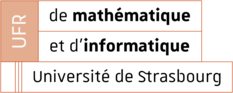
\includegraphics[scale=1.]{img/logo_UFR_2.png}}
\end{figure}

\pagenumbering{roman}

\newpage
% \addcontentsline{toc}{section}{Table des matières}
\renewcommand{\contentsname}{Table des matières}
\tableofcontents

\newpage
\addcontentsline{toc}{section}{Liste des figures}
\renewcommand{\listfigurename}{Liste des figures}
\listoffigures

\newpage
\pagenumbering{arabic}
\vspace*{0.01cm}
\section*{Introduction}
L'objectif du projet est de réaliser un système de recherche d’information dans une collection de descriptions de films publiées sur Allociné.\\
Le projet se décompose en deux parties:
\begin{itemize}
\item  Prédiction du genre des films par TAL
\item Visualisation des résultats
\end{itemize}

L'ensemble des fichiers (jeux de données et notebooks) utilisés sont accessibles sur GitHub: \url{https://github.com/FABallemand/ProjetTAL}

\section{Analyse et Pré-traitement des Données}
Dans un premier temps, les données d'entraînement (\textit{allocine\_genres\_train.csv}) peuvent être chargées grâce à la fonction \textsf{read\_csv} de la bibliotèque Pandas \cite{pandas} en précisant le séparateur (\textsf{sep=","}). L'utilisation des méthodes \textsf{head}, \textsf{tail}, \textsf{describe}, \textsf{info} et \textsf{hist} permettent de visualiser et comprendre les données contenues dans le jeu de données complet.

Dans le cadre de ce projet seules les données contenues dans les colonnes \textit{titre} et \textit{synopsis} seront utilisées pour déduire la valeur contenue dans \textit{genre}. Le jeu de données peut être réduit à ces trois features.\\
Etant donné que les données vont être utilisées pour de l'apprentissage automatique, il faut vérifier s'il y a des valeurs manquantes. Les méthodes \textsf{isna} et \textsf{sum} ne révèlent aucune valeur manquante dans les données d'entraînement.\\
La proportion des classes dans le jeu de données peut avoir un impact sur l'apprentissage. Les classes ayant un effectif plus faible seront généralement moins bien "apprises". La figure \ref{value_counts} montre que les classes n'ont pas toutes la même proportion dans le jeu de données: il y a beaucoup d'individus de la catégorie \textit{drame} alors que les classes \textit{biopic}, \textit{documentaire} et \textit{historique} sont très peu représentées.

\begin{figure}
    \center
    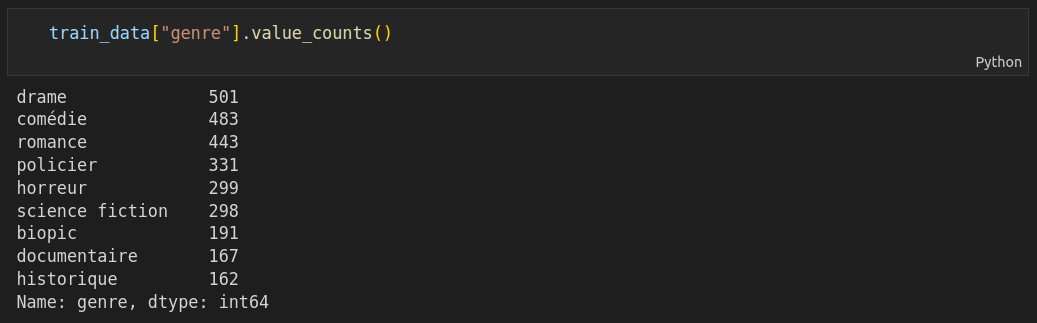
\includegraphics[scale=.3]{img/value_counts.png}
    \caption{Effectifs des classes dans les données d'entraînement}
    \label{value_counts}
\end{figure}

Après de nombreuses expériences, il s'avère que rééquilibrer les classes par \textit{oversampling}, c'est à dire: dupliquer des individus des classes les moins représentées, donne de meilleurs résultats quelque soit la méthode utilisée. (Figure \ref{confusion})\\
\textbf{Dans tout la suite,} les résultats présentés correpondront aux résultats obtenus avec le jeu de données d'entraînement rééquilibré par \textit{oversampling} à l'aide de l'objet \textsf{RandomOverSampler} de la bibliotèque Imbalanced-learn \cite{imbalanced_learn}.

\begin{figure}
    \centering
    \subfloat[\centering Matrice de confusion du modèle de régression logistique avec des classes déséquilibrées]{{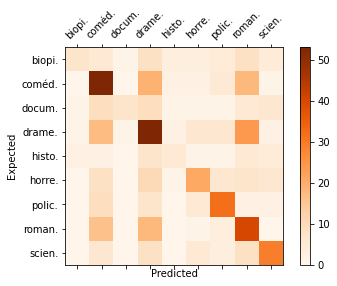
\includegraphics[width=5cm]{img/imbalanced.png}}}
    \qquad
    \subfloat[\centering Matrice de confusion du modèle de régression logistique avec des classes équilibrées par oversampling]{{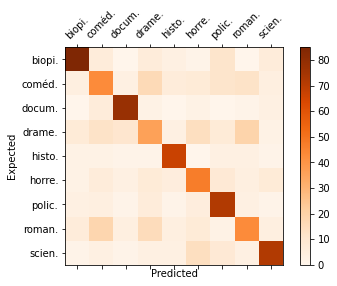
\includegraphics[width=5cm]{img/balanced.png}}}
    \caption{Comparaison des matrices de confusion pour des données déséquilibrées et équilibrées: les classes les moins représentées dans le jeu de données d'entraînement sont moins bien apprises lorsque les classes sont déséquilibrées.}
    \label{confusion}
\end{figure}

\noindent
\begin{minipage}[!hc]{0.12\textwidth}
   \textbf{Remarque}
\end{minipage}
\vrule\enskip\vrule\quad\begin{minipage}{\dimexpr 0.87\textwidth-0.8pt-1.5em}
Le jeu de données d'entraînement contient trop peu de données pour effectuer un équilibrage des classes par \textit{undersampling}, c'est à dire: supprimer des individus des classes les plus représentées. Les résultats obtenus avec cette méthode étaient généralement moins bons que sans équilibrage.
\end{minipage}

\section{Méthodes Basiques}

\subsection{Pré-traitement des Données}
Il est possible de mettre en place une pipeline (Figure \ref{pipeline_1}) afin de vectoriser les données d'apprentissage et d'en extraire des informations statistiques.\\
Dans cette pipeline, les données déjà tokénisées vont être lemmatisées et vectorisées selon la méthode TF-IDF en supprimant les stop-words. Puis des objets \textsf{Functiontransformer} et \textsf{DictVectorizer} de la bibliotèque Scikit-learn \cite{scikit_learn} vont être utilisés pour obtenir les valeurs statistiques telles que la longeur du synopsis en nombre de mots et en nombre de phrases. Un \textsf{MinMaxScaler} est utilisé pour normaliser ces données afin qu'elles aient le même poids lors de l'apprentissage.

\begin{figure}
    \center
    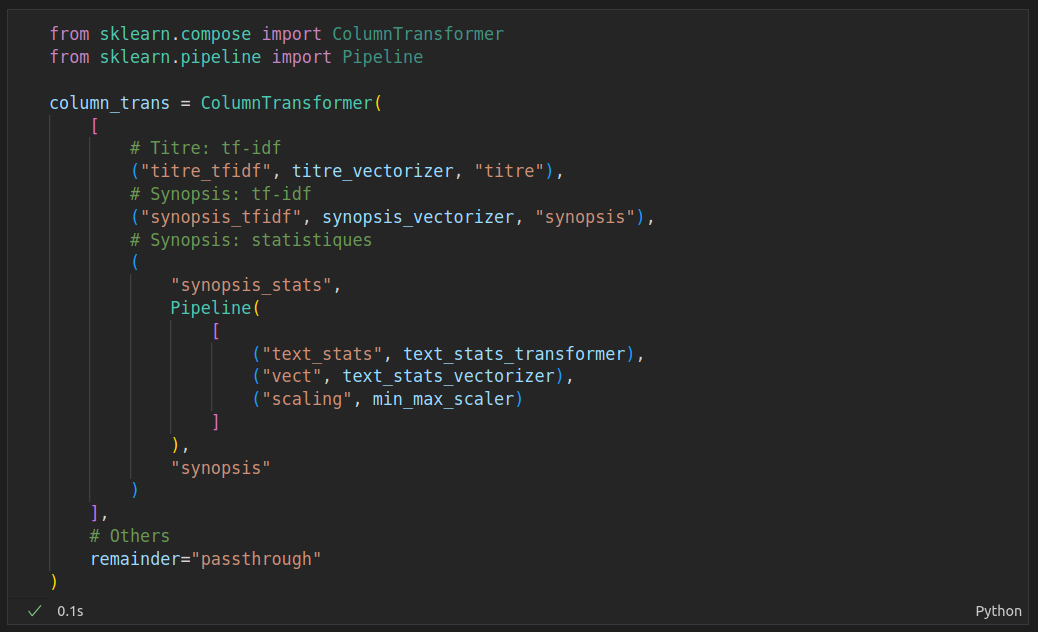
\includegraphics[scale=.3]{img/pipeline_1.png}
    \caption{Pipeline de pré-traitement des données}
    \label{pipeline_1}
\end{figure}

\subsection{Apprentissage Simple}
Avant tout apprentissage supervisé, il faut définir un jeu d'apprentissage et un jeu de test avec par exemple la méthode \textsf{train\_test\_split} de Scikit-Learn en spécifiant la proportion du jeu de données sélectionnée pour les données de test (typiquement: \textsf{test\_size=0.2}) et précisant \textsf{shuffle=True} pour que les données ne soient pas sélectionnées séquentiellement (ce qui pourrait impacter le résultat si le jeu de données est trié par classes).

\noindent
\begin{minipage}[!hc]{0.12\textwidth}
   \textbf{Remarque}
\end{minipage}
\vrule\enskip\vrule\quad\begin{minipage}{\dimexpr 0.87\textwidth-0.8pt-1.5em}
Le jeu de données \textit{allocine\_genres\_test.csv} correspond au jeu de validation qui ne sera utilisé qu'après avoir définitivement choisi la méthode de prédiction.
\end{minipage}

Il est alors possible de créer une nouvelle pipeline pour automatiser le pré-traitement et l'apprentissage (Figure \ref{pipeline_2}).

\begin{figure}
    \center
    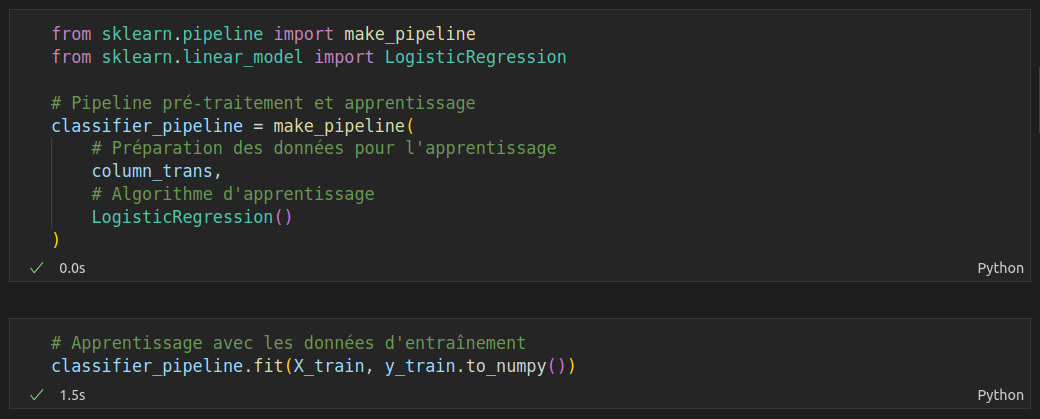
\includegraphics[scale=.3]{img/pipeline_2.png}
    \caption{Pipeline d'entraîenement d'un modèle de régression logistique}
    \label{pipeline_2}
\end{figure}

On peut ensuite faire des prédictions sur le jeu de test avec la méthode \textsf{predict} pour évaluer le modèle. Ce modèle de régression logistique donne une précision de 0.6 et un rappel de 0.61 (donc un score f1 de 0.6).

\subsection{Apprentissage par Plis et Comparaison des Algorithmes}
Comme vu précédemment, la taille et les individus sélectionnés pour entrainer le modèle peuevent avoir une influence sur la qualité de l'apprentissage. Pour contrer ce biais on peut utiliser des plis pour l'apprentissage: au lieu de diviser les données d'entraînement en un jeu d'entrainement et un jeu de test, on peut diviser les données d'entraînements en plusieurs plis qui seront tour à tour des données d'entraînement ou de test. Cela permet d'obtenir une idée de la performance moyenne du classifieur. On utilise la méthode \textsf{StratifiedKFold} de Scikit-Learn qui a la particularité de conserver la proportion d'individus de chaque classe dans les plis.

En utilisant cette méthode, on peut comparer le modèle de régression logistique avec d'autres algorithmes. Les meilleurs résultats proviennent d'un modèle de forêt aléatoire (précision proche de 0.7). (Figure \ref{comparaison})

\begin{figure}
    \centerz
    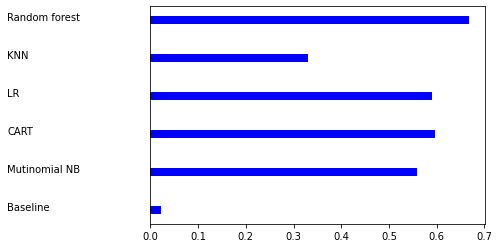
\includegraphics[scale=.6]{img/comparaison.png}
    \caption{Précision de différents algorithmes lors d'un apprentissage par validation croisée avec 5 plis}
    \label{comparaison}
\end{figure}

% \input{src/gen.tex}

\section*{Conclusion}
Avec le temps et la puissance de calcul à disposition, le meilleur modèle pour
la classification des films semble être le réseau neuronal convolutif. Il offre
des résultats proches du BILSTM pour un temps d'entraînement significativement
plus faible.

\begin{table}[]
    \begin{tabular}{|l|l|l|l|l|}
        \hline
        Modéle    & Radom Forest & CNN     & BILSTM  & Transformer \\
        \hline
        Précision & 66\%         & 72.91\% & 74.51\% & ???         \\
        \hline
    \end{tabular}
    \caption{Résultats des modèles testés}
    \label{accuracy}
\end{table}

En entrainant le même modèle avec l'ensemble des données du jeu d'entraînement et en testant sur l'ensemble des données du jeu de test, on observe une précision d'environ 50\%.\\
Ce niveau de précision semble faible, cependant si on observe le vecteur de probabilités à la sortie des couches denses, dans 80\% des cas le CNN place le genre attendu dans les trois premiers genres prédits (et il semble faire des erreurs sur les genres qui sont proches par exemple \textit{science-fiction} et \textit{historique} sont rarements ensembles dans les trois premires genres).

Les résultats obtenus avec le modèle choisi ne sont peut-être pas les meilleurs résultats qu'il est possible d'obtenir sur ces jeux de données. Voici quelques pistes de recherche que nous aurions aimé explorer:
\begin{itemize}
    \item Transformer
    \item Grid search avec différents pré-traitement des données (tokénisation, vectorisation...) sur les différents modèles
    \item Méthodes d'intelligence collective (exemple: entraîner plusieurs CNN et efffectuer un vote pour prédire le genre)
\end{itemize}

Après avoir enregistré les prédiction dans un fichier au format \textsf{csv}, les résultats obtenus peuvent être parcourus et analysés au moyen d'une interface web basée sur Solr \cite{solr}. L'utilisation des panneaux latéraux permet de filtrer les résultats des requêtes. (Figure \ref{solr})

\begin{figure}
    \center
    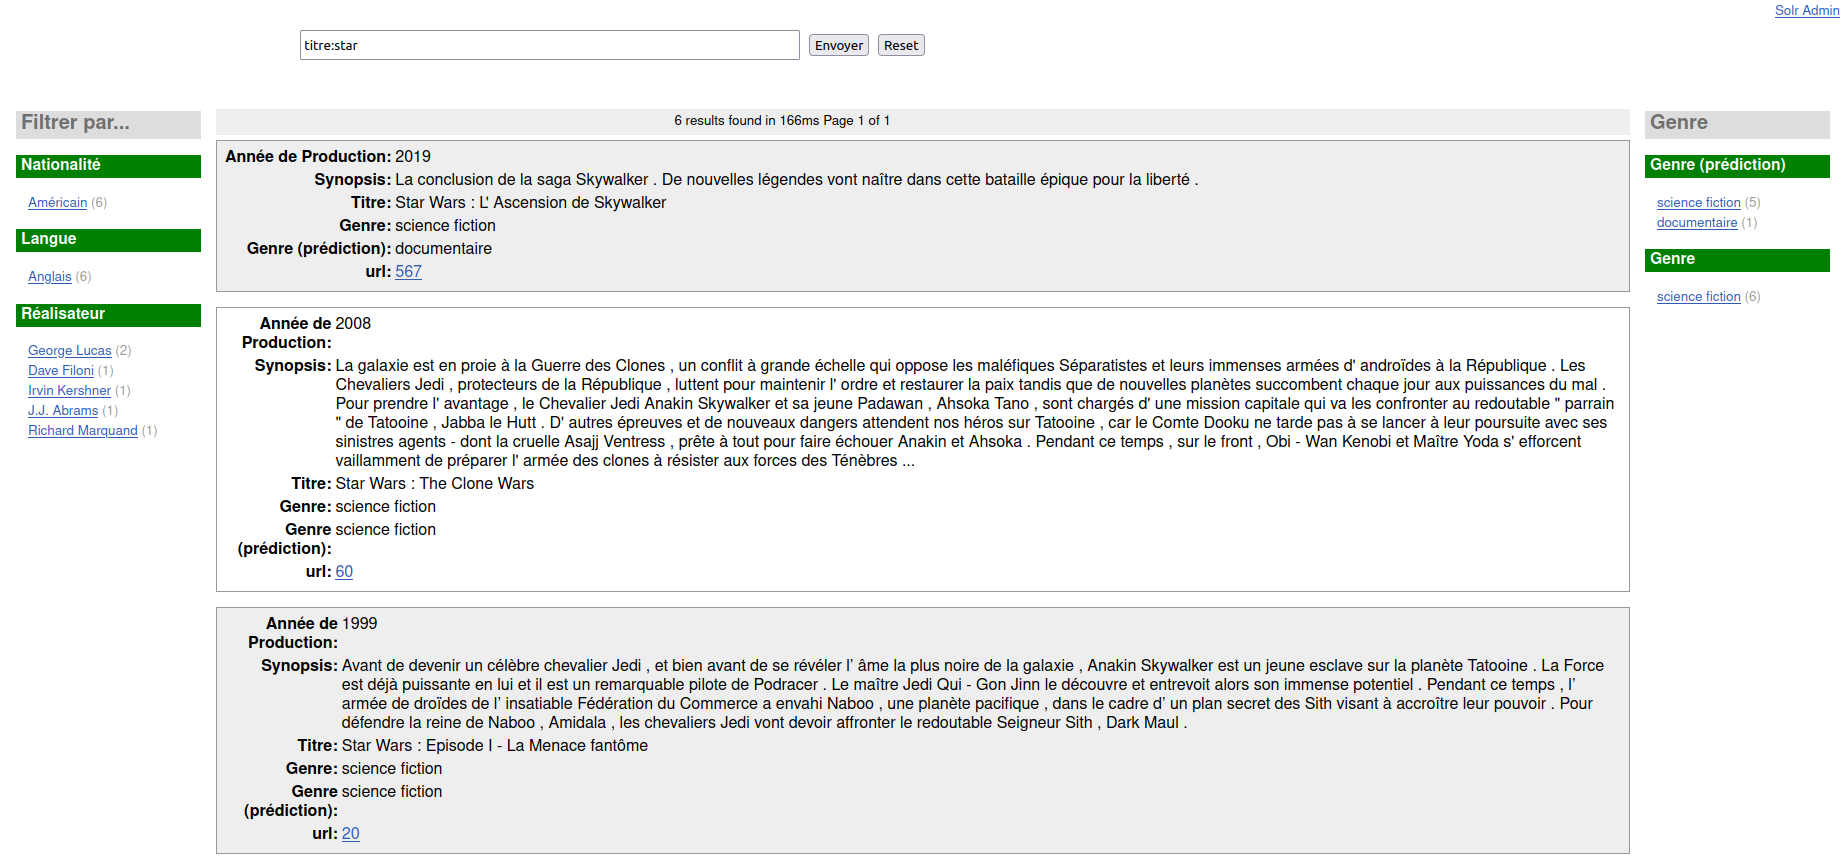
\includegraphics[scale=.25]{img/solr.png}
    \caption{Interface web Solr pour une requête sur le mot \textit{star}}
    \label{solr}
\end{figure}



\newpage
\addcontentsline{toc}{section}{Bibliographie}
\renewcommand{\refname}{Bibliographie}
\bibliographystyle{plain}
\bibliography{bibliography}

\end{document}